\section{Introduction}

Atom-to-atom mapping connects a reaction's endpoint structures to an account of which atoms persist and which relationships change. The selected correspondence influences reaction-center identification, template extraction, and endpoint preparation for computational reaction studies. Curated benchmarks also show that evaluation requires careful treatment of molecular representation, incomplete records, and chemically equivalent assignments~\citep{lin2022}.

Modern approaches provide efficient mappings through distinct routes. RXNMapper extracts correspondence information from attention in a language model trained on unannotated reactions~\citep{schwaller2021}. LocalMapper learns from chemist-labeled reactions through a human-in-the-loop procedure~\citep{chen2024}. SLAPMapper combines Weisfeiler--Lehman-like label refinement with sequential linear assignment problems, exposing alternative mappings and a general graph-matching interface~\citep{koda2025}. Its efficiency and alternative outputs make it a particularly relevant comparator for an explicit search over mapping possibilities.

For mechanistic exploration, an alternative can be useful even when it is not the lowest-edit output. Conversely, many atom-index permutations need not represent distinct chemistry. A useful search representation must distinguish alternative structural decisions from redundant realizations and preserve correlations between atoms that move together. Ranking one representative cannot characterize the entire family it represents.

Here we develop a fragment-growth approach in which fragments are constructed incrementally from weighted endpoint graphs. Candidate placements evolve during growth, and distinct saturated placements define branches for subsequent decisions. Candidate canonicalization, conservative reconvergence of cumulative states, and downstream family containment address redundancy at different levels. Seed orderings and single-edge sweeps diversify the trajectories. We evaluate reference recovery, the cost of seed diversity, and retained alternatives on native coordinate and bond-order inputs, while keeping these metrics distinct.

\section{Methods}

\subsection{Weighted endpoints and mapping scope}

Let $V_R,V_P$ denote source and target atom sets, $Z_R,Z_P$ their element labels, and $W_R,W_P$ their symmetric bond-weight matrices. The search constructs an injective element-compatible correspondence $m:D_R\subseteq V_R\rightarrow V_P$. Equal-composition endpoints admit a full bijection; partial coverage remains explicit for incomplete records. Hydrogen atoms participate in search. Coordinates accompany native endpoints but do not determine the growth decisions considered here.

An active graph is obtained using bond floor $b=0.2$. Extension checks use the supplied numerical weights with tolerance $\tau$. Golden inputs use formal bond-order values from molecular records; the coordinate collection uses cached continuous Wiberg bond-order (WBO) matrices. These representations are distinct. Continuous fragment growth refers to continued incremental extension while compatible placements evolve; the method also accepts continuous weights.

\subsection{Continuous fragment growth}

A fragment starts at one source atom with a compressed collection of compatible target placements. Its frontier is a priority queue of active source edges, ordered by decreasing weight with deterministic tie handling. For a proposed source atom $n$ and target image $v$, a placement must preserve element identity and injectivity and satisfy, for every active edge $(n,u)$ to the current fragment $F$,
\begin{equation}
W_P[v,m(u)]\geq b,\qquad |W_R[n,u]-W_P[v,m(u)]|\leq\tau.
\label{eq:extension}
\end{equation}
All such edges are checked, rather than only the queue edge initiating the attempt. Source nonedges are not local negative constraints; additional target bonds can later be classified as formed bonds.

A candidate stores a representative mapping, unresolved assignment blocks, and symmetry evidence. If an extension touches an unresolved block, compatibility requires a jointly consistent injective assignment. A failed arbitrary representative is insufficient to reject the compressed candidate. This local support calculation has an implementation budget and is distinct from enumerating complete mappings.

When at least one extension survives, growth commits the enlarged fragment and continues with the surviving placements. A unique placement does not end growth early. If no placement supports an extension, that edge becomes a deferred boundary and growth continues elsewhere. Reaching an already mapped atom triggers an attempt to absorb its entire locked island, verifying the added relationships and respecting existing assignments.

At saturation, distinct placements yield separate branches of the whole-mapping search. Alternatives therefore exist within a growing fragment and among sequences of saturated fragment decisions. Growth is conditional and greedy along each trajectory: accepting an extension filters candidates that cannot support it. Every possible fragment boundary is not explored, so seed orderings and cut conditions affect coverage.

\begin{figure}[tb]
\centering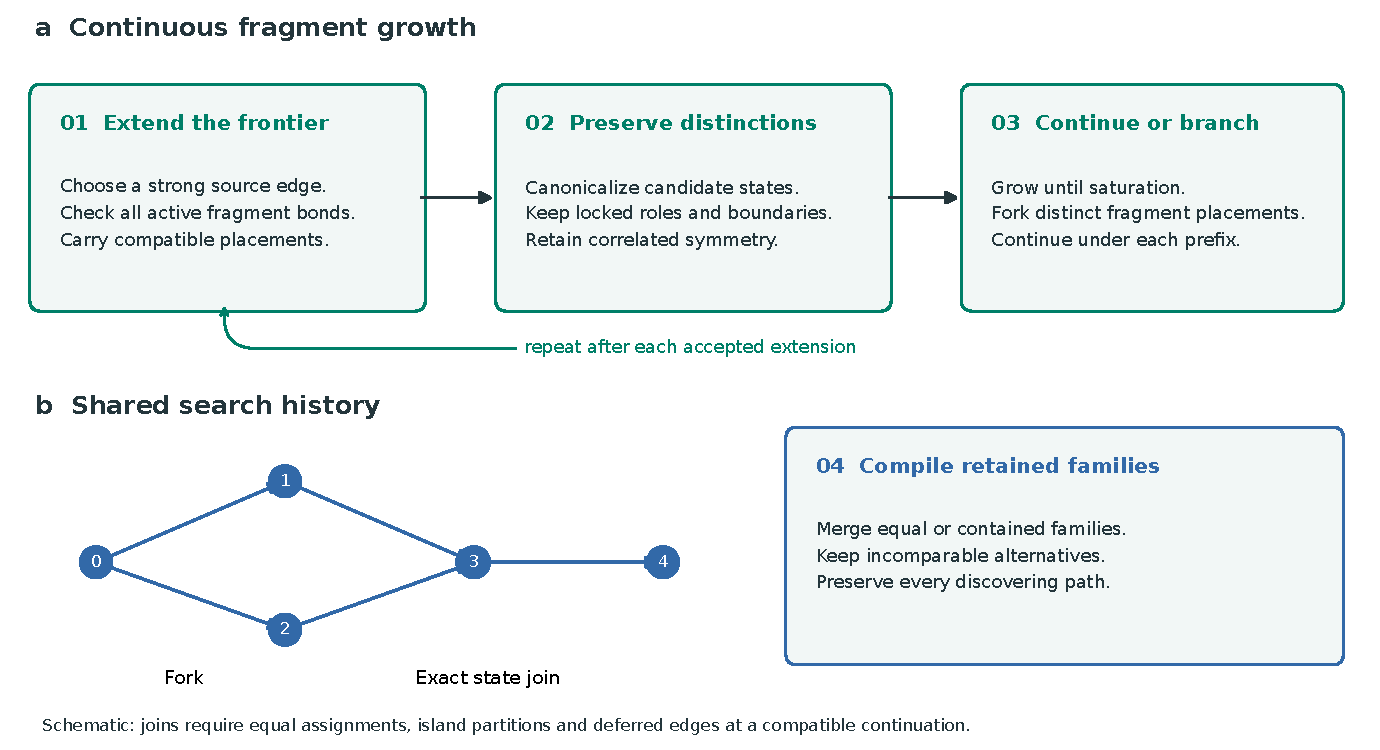
\includegraphics[width=\linewidth]{figs/fig1_algorithm.pdf}
\caption{\textbf{Continuous growth and shared search history.} (a) Extension alternates with candidate canonicalization until saturation; distinct placements continue as separate mapping branches. (b) Schematic fork and reconvergence. Joins require equal cumulative states at a compatible continuation within one context. This diagram is conceptual, not a measured reaction trajectory.}
\label{fig:algorithm}
\end{figure}

\subsection{Context-preserving deduplication}

Deduplication operates at three levels (\Cref{fig:algorithm}). During local growth, colored graph certificates encode target structure, candidate roles, assignment pools, and locked images. Canonical labeling uses nauty~\citep{mckay2014}. The configured bond-weight coloring defines the symmetry model; numerical compatibility remains subject to \Cref{eq:extension}. Deferred edges and the current one-hop boundary preserve distinctions relevant to later growth. Merging retains symbolic variation without computing a full automorphism group at every extension. Exact conditioned generators are finalized on recorded transitions needed by the returned results.

At the whole-mapping level, cumulative state contains the representative assignment, normalized island partition, and deferred edges. Equal states can reconverge at the same continuation step under the same cut/seed context. Both incoming histories remain connected to their shared continuation in a directed acyclic graph. Equal mappings alone do not justify discarding different fragment relations; different cut contexts are not joined solely because assignments agree.

For completed supported relations, downstream compilation represents a family by a representative $m_0$ and permitted target actions $G$:
\begin{equation}
\mathcal F=\{g\circ m_0:g\in G\}.
\end{equation}
Equality and containment checks merge equal or subsumed families while retaining provenance; incomparable families remain distinct. These checks require the complete relation and do not justify a more aggressive quotient of incomplete states. Atom orbits are summaries, not independent permissions to permute atoms. An earlier fragment action must transport dependent later assignments and generators together. Optional mechanism grouping and geometry-based selection consume these relations downstream.

\subsection{Seed orderings, sweeps, and budgets}

One benchmark seed setting denotes one ordering of source atoms, not one atom-pair assignment. The scheduler visits eligible seeds under each branch's constraints, repeating passes while progress remains possible. A sweep includes the uncut graph and each eligible single-edge deletion. Cuts change growth constraints; event evaluation uses original endpoint matrices. Deterministic cut-specific streams derive from root seed 42.

The seed ablation retains both directions, explicit H, $\tau=1.0$, and branch cap 100 while varying only the number of orderings per cut among 1, 2, 3, and 10. Shorter lists are prefixes of the same deterministic sequence. Bidirectional output is a union of independently returned alternatives, without splicing branches.

Caps apply to live compressed candidates during growth and to post-deduplication branch admission. An overflowing parent subtree is discarded while siblings survive; exactly 100 branches are allowed. A cap can coexist with a complete mapping. The seed experiments use 300-second search watchdogs and separate 240-second analysis watchdogs. Bounded symbolic checks can remain unresolved even when analysis exits normally.

A separate adaptive no-sweep experiment uses a balanced seed agenda with saved budgets of 400, 1,600, and 6,400 growth operations and a 30 CPU-second soft limit per direction. It retains the native growth cap of 100 but replaces the synchronized frontier cap with an agenda budget. Its last saved checkpoint defines output. This changes the search policy as well as sweep usage; it is not an isolated cut ablation.

\subsection{Golden benchmark and reference recovery}

We use all 1,851 original Golden records~\citep{lin2022}, with dataset revision \texttt{793475e}. Reference labels are removed before search; records are not removed or repaired to improve compatibility. Explicit-H expansion and formal bond-order matrices provide AAM inputs. No coordinate optimization is performed for Golden.

Correctness is equality of the annotated heavy-atom correspondence relation, including unmatched atoms, modulo chemical automorphisms of both endpoints. Evaluator colors retain element, charge, isotope, hydrogen count, and stereochemistry, with bond-order and bond-stereochemistry relations. Returned chemistry must remain unchanged. H identity is not scored as reference provenance, although H participates in search.

Recovery requires a verified reference witness among retained alternatives. Verified absence concerns saved output. Unresolved verification establishes neither recovery nor absence. Failures and unknowns remain in the denominator. Family recovery, first-output correctness, representative top-$k$, and event-window recovery are distinct metrics.

\subsection{SLAP comparisons}

We test SLAPMapper 1.0.0 at revision \texttt{ea248fd}, retaining native alternatives~\citep{koda2025}. The new sweep uses one original ordering, both directions, and binary and weighted modes. Each variant runs the uncut input and every single source-edge deletion, rebuilding initialization after each cut. Explicit H and native element-balancing placeholders remain. Output labels are restored to the original endpoints before evaluation.

Cuts perturb SLAP's graph and objective, rather than its internal assignment or pruning rules; their effect is not assumed identical to AAM's fragment constraints. References never select cuts or stop searches. Each case/direction/mode variant has a 300-second watchdog across its cuts. We distinguish the uncut control, standalone sweep, and union with an earlier expanded-SLAP experiment. Default competitors appear in the supporting information without equating their cardinalities or search budgets to the sweeps.

\subsection{Native XYZ/WBO collection and shared score}

The second collection comprises 140 selected elementary steps with 18--137 explicit atoms per endpoint, including multicomponent and organometallic structures. Each pair has equal elemental composition. No annotated reference mappings exist. Searches consume original coordinates and cached WBOs without previous predictions or reference TS structures.

The native comparison uses AAM on WBO graphs and SLAP's \texttt{map\_3d} interface on original component XYZ files, with native distance-based binary connectivity and bond scale 1.2. These workflows have different representations. Saved full assignments are then scored on the same WBO matrices, including H. A bond is present above 0.2; a preserved bond contributes an order-change event when its WBO difference exceeds 0.5:
\begin{equation}
E(m)=N_{\mathrm{broken}}(m)+N_{\mathrm{formed}}(m)+N_{\mathrm{order\ changed}}(m).
\end{equation}
This shared score differs from optional metal-specific thresholds elsewhere in the software. SLAP H assignments are refined within saved label pools. AAM minima concern saved representatives, not a certified optimum over all compressed families.

Heavy classes are compared using exact graph certificates with score-preserving endpoint equivalences. Missing representatives are queried against compressed families when the budget permits; unresolved membership stays unknown. The main comparison uses tolerance 1.0, ten orderings, and cap 100 throughout. A previous case-123 cap-200 follow-up remains separate.

\subsection{Compute accounting and experimental versions}

The seed ablation uses frozen native-reuse engine \texttt{98b01b1}, with eight CPUs per directional AAM call. The timing subset contains 1,807 Golden reactions completed by every configuration. Instrumented parent-plus-child AAM CPU excludes measured saving/loading but includes process and communication setup. SLAP's workflow timer excludes worker startup. Interrupted work without final readings is excluded from this paired successful-work comparison. These are scoped compute measurements, not total resources or equal-resource latency. Recovery always uses 1,851 records.

Earlier engine \texttt{bb0a7d7} provides a separate frozen recovery and concrete-candidate collection experiment. Its outputs are not unioned into the seed ablation. Saved artifacts include inputs, source hashes, cut archives, statuses, witnesses, and timings. Figures are generated from machine-readable report snapshots.

\section{Results}

\subsection{Sweeping improves SLAP recovery}

The uncut control recovers 1,661/1,851 references (89.74\%) across both directions and bond modes. The sweep raises recovery to 1,795 (96.97\%), adding 134 cases (\Cref{fig:golden}). Binary sweeps recover 1,785 and weighted sweeps 1,762; the modes provide complementary outputs.

Earlier expanded SLAP recovers 1,691 (91.36\%). Its union with the new sweep recovers 1,797 (97.08\%), a separate result. Of 54 remaining cases in that union, 50 were fully swept and valid and four were incomplete. Completing those four alone cannot bring this policy to 99\%. This does not bound other SLAP policies.

Of 355,104 planned calls, 352,210 are recorded: 352,208 succeeded and two had upstream exceptions. No returned mapping fails strict format and endpoint-preservation validation. There are 65 watchdog-limited variants among 7,404 case/direction/mode variants; their completed cuts remain included.

\begin{figure}[tb]
\centering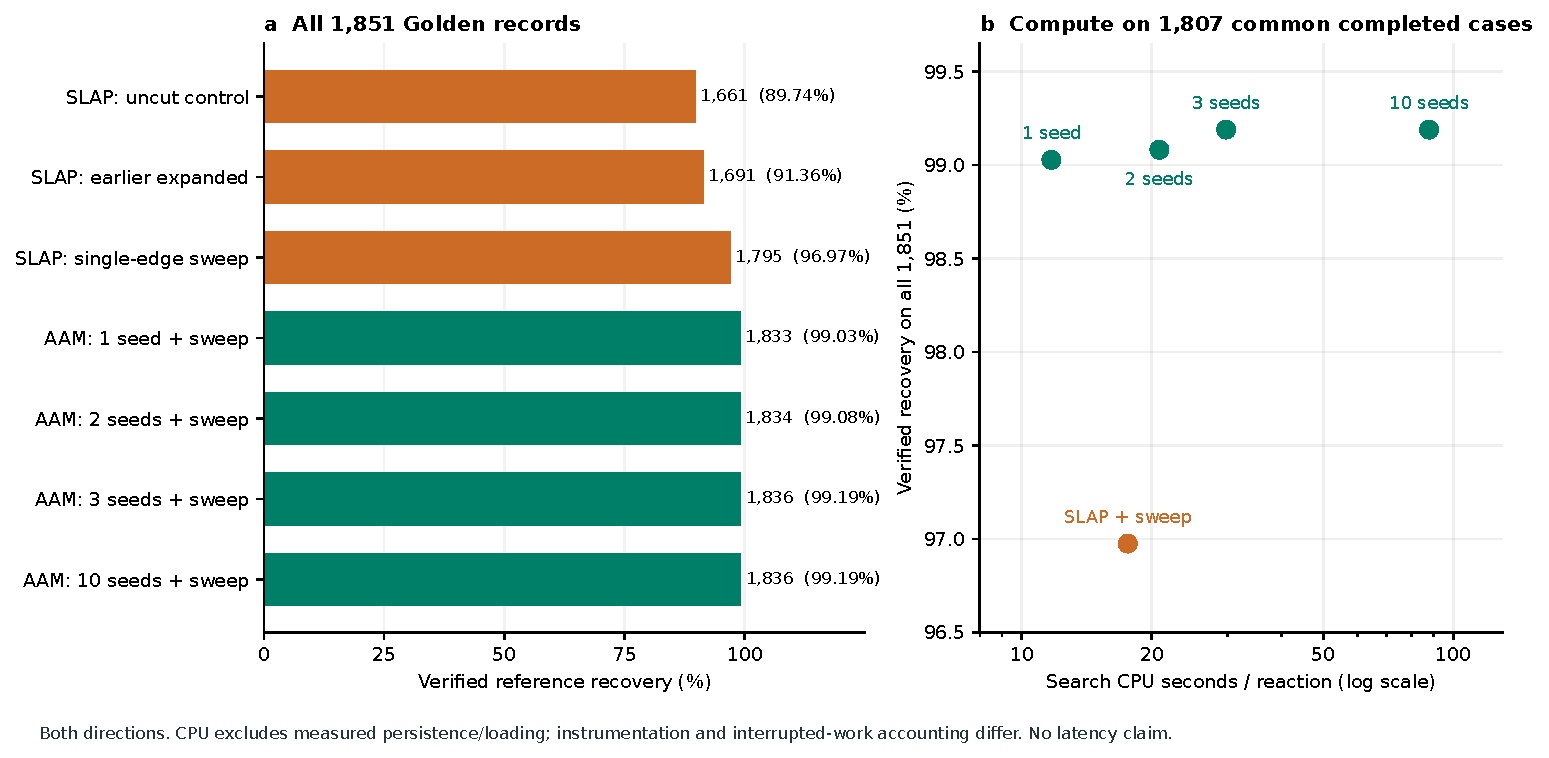
\includegraphics[width=\linewidth]{figs/fig2_golden.pdf}
\caption{\textbf{Golden recovery and compute.} (a) Recovery among retained alternatives on all 1,851 records. SLAP control and sweep use both directions and bond modes; earlier expanded SLAP has a separate ordering budget. (b) Full-denominator recovery versus mean CPU on 1,807 mutually completed reactions. The horizontal axis is logarithmic. Persistence/loading are excluded, instrumentation differs, and interrupted work is omitted. This is not a latency comparison.}
\label{fig:golden}
\end{figure}

\subsection{Few seed orderings retain high recovery}

One ordering per cut recovers 1,833 references (99.03\%), with 17 absences and one unknown. Two recover 1,834 (99.08\%), and three recover 1,836 (99.19\%). The ten-order baseline also verifies 1,836, although case sets and unknown outcomes differ (\Cref{tab:seeds}). Each fresh one-, two-, and three-order experiment completes all 3,982 directional searches and 3,982 analysis processes across both collections, without a hard watchdog.

\begin{table}[tb]
\centering\small
\caption{\textbf{Seed ablation under the frozen native-reuse engine.} Outcomes use all 1,851 Golden records. CPU sums both directions and all cuts on the same 1,807 completed reactions.}
\label{tab:seeds}
\begin{tabular}{lrrrrr}\toprule
Configuration & Recovered & \% & Absent & Unknown & CPU s/reaction\\\midrule
1 seed order & 1,833 & 99.03 & 17 & 1 & 11.72 \\
2 seed orders & 1,834 & 99.08 & 14 & 3 & 20.85 \\
3 seed orders & 1,836 & 99.19 & 10 & 5 & 29.77 \\
10 seed orders & 1,836 & 99.19 & 5 & 10 & 87.87 \\
\bottomrule\end{tabular}

\end{table}

Mean paired costs are 11.72, 20.85, 29.77, and 87.87 CPU-seconds per reaction for one, two, three, and ten orderings. One ordering costs 7.50-fold less than ten. SLAP's sweep uses 17.62 seconds per reaction, giving a one-order AAM/SLAP ratio of 0.665 within the recorded scope.

Equal totals do not imply identical coverage. Relative to ten orders, one order no longer verifies seven cases, including one now unknown, but verifies four previously unknown cases. Those gains reflect completed search or verification, not a superset explored by fewer orderings. No cross-setting union contributes to reported recovery.

\subsection{Adaptive no-sweep search changes coverage}

The separate adaptive no-sweep policy verifies 1,723/1,851 Golden references (93.08\%) bidirectionally, with 33 verified absences and 95 unknowns. All 3,702 directional Golden searches complete under their budgets. On the 140 coordinate pairs, it returns full mappings for every case and matches the original ten-order sweep's best saved score in 138 cases; two scores are worse. Thus high mapping availability and score agreement on coordinate inputs do not establish equivalent reference recovery or retained families. This experiment does not isolate the effect of removing cuts from the original scheduler.

\subsection{Concrete recovery extends beyond minimum event score}

The earlier publication engine verifies 1,839/1,851 references (99.35\%) bidirectionally, with nine absences and three unknowns. Its representative top-1 result is 1,434/1,851 (77.47\%). This gap illustrates why family recovery cannot be presented as single-answer accuracy.

Extraction from those archives recovers all 1,839 as concrete candidates within six additional bond events of the best collected candidate (\Cref{fig:windows}). At minimum score alone, recovery is 1,692 (91.41\%); allowing two additional events gives 1,817 (98.16\%). This is an event window, not top-$k$. Extraction remains bounded: 20,916 visited families are unresolved and only 409 bidirectional records have exhaustive extraction certificates. The result shows useful higher-event candidates without establishing that all are chemically plausible.

\begin{figure}[tb]
\centering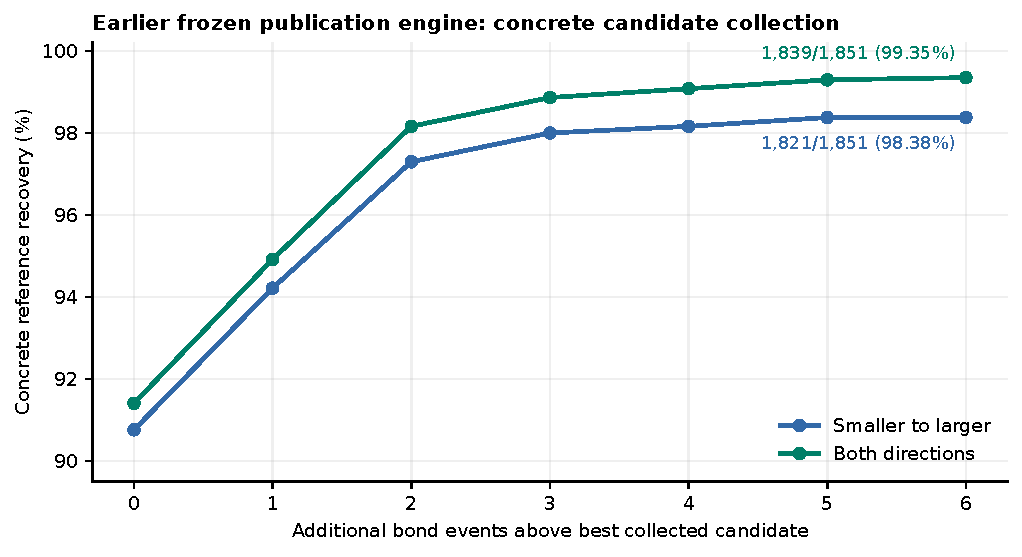
\includegraphics[width=.82\linewidth]{figs/fig4_event_windows.pdf}
\caption{\textbf{Recovery among collected concrete candidates.} This uses the earlier publication engine, separately from the seed ablation. Event windows are relative to the best collected score at maximum coverage. All 1,851 records remain in the denominator. Extraction does not enumerate every represented mapping.}
\label{fig:windows}
\end{figure}

\subsection{Coordinate inputs retain distinct alternatives}

All four seed settings return full explicit-atom mappings for all 140 XYZ/WBO cases. Best saved scores for one, two, and three orders agree with ten in 139 cases. In case 123 the counts are respectively 27, 25, 25, and 19. Mapping availability is stable under seed reduction, whereas representative score can change.

In the separate tolerance-1.0 comparison with native XYZ SLAP, at ten orders and strict cap 100, best scores tie in 133 cases; AAM is lower in six and SLAP in one (\Cref{fig:holdout}). The prior cap-200 follow-up reduces case 123 from 19 to 3 events, yielding 134 ties, six AAM-lower, and zero SLAP-lower. The fixed-cap comparison remains the primary scope.

Of 176 SLAP heavy classes, 159 are represented in strict-cap AAM families, 12 are excluded from those archives, and five are unresolved. Conversely, 97 cases have an extra AAM heavy pattern absent from saved SLAP at the lowest observed AAM score. This rises to 99 within one additional event, 132 within two, and 138 within five. Score agreement does not imply equal families. Neither method is shown to contain the other's complete output space; missing annotations prevent a chemical-accuracy claim.

\begin{figure}[tb]
\centering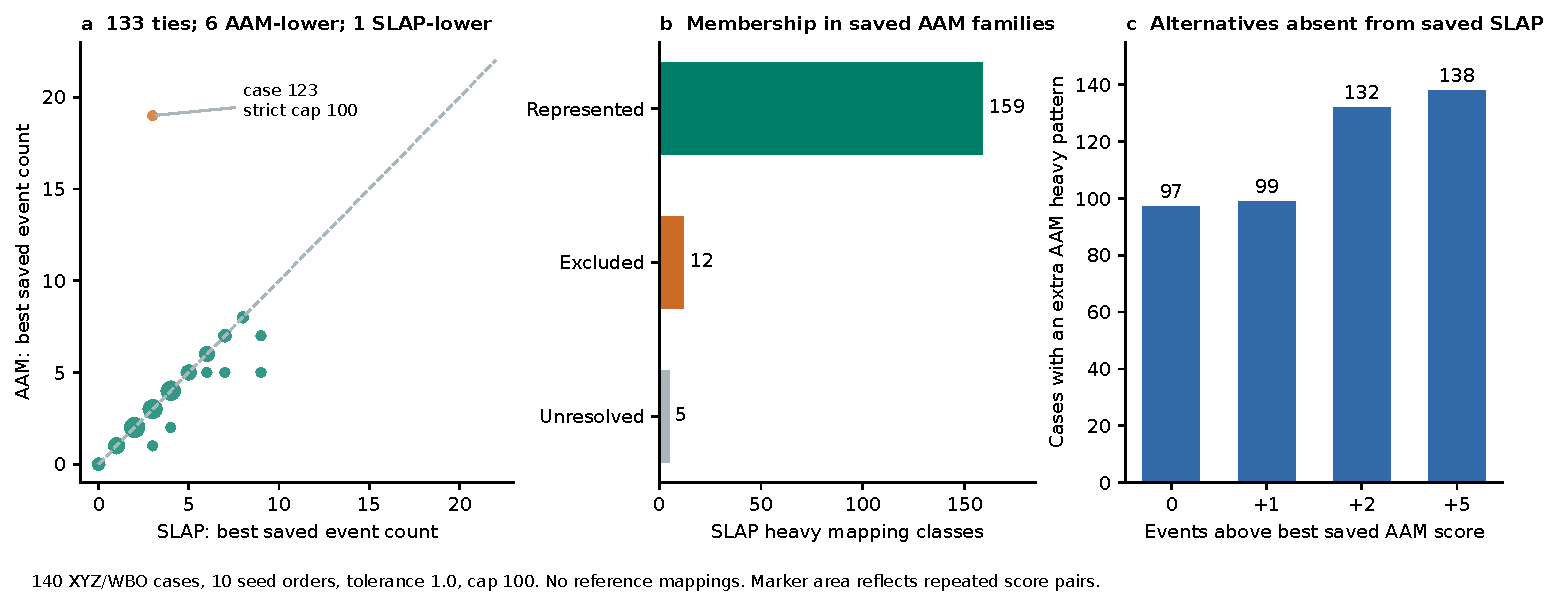
\includegraphics[width=\linewidth]{figs/fig3_holdout.pdf}
\caption{\textbf{Saved outputs on 140 XYZ/WBO cases.} All panels use tolerance 1.0, ten orders, and strict cap 100. (a) Best representative scores under a shared full-H WBO score; the dashed line denotes equality. (b) Membership of 176 SLAP heavy classes in saved AAM families. Exclusion concerns these archives; unknowns are separate. (c) Cases with an extra AAM heavy pattern absent from saved SLAP within each event window. No reference mappings exist for this collection.}
\label{fig:holdout}
\end{figure}

\subsection{Recorded growth exposes mapping decisions}

\Cref{fig:growth} illustrates an uncut replay on 18-atom carbocation case 64. The first ordering starts at source atom 13 with five compressed candidates. Growth increases the count to 42 before additional context reduces it to two distinct saturated placements. Ambiguity can expand and contract during growth. Candidate counts measure compressed states, not atom permutations.

Movie 1 and the interactive viewer replay this trajectory and expose its two terminal representatives. Movie 2 follows TEMPO case 1 through eight deferred-boundary observations and four fragment decisions. Both use one ordering, no sweep, tolerance 1.0, and cap 100 with the event-enabled Python path of the frozen source. These illustrative runs do not contribute to benchmark totals or timing. Animation time indexes algorithm events, not physical reaction time.

\begin{figure}[tb]
\centering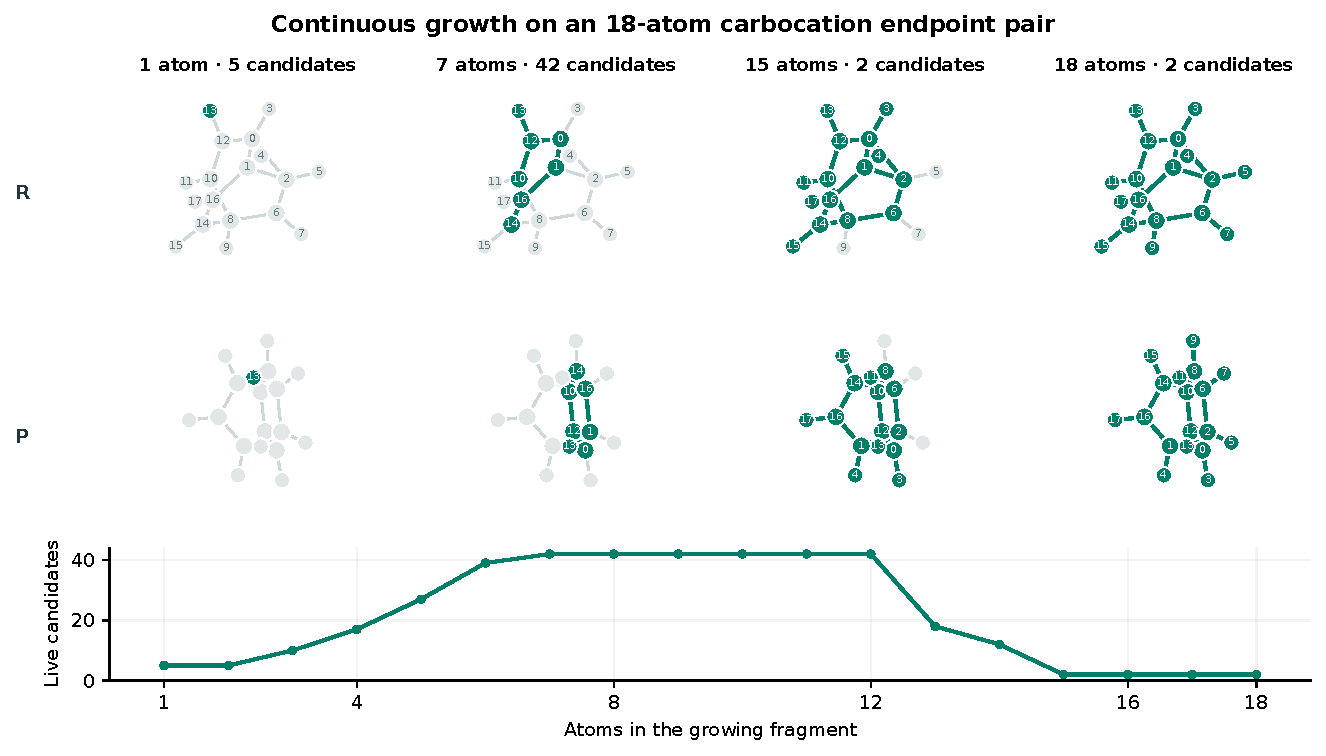
\includegraphics[width=\linewidth]{figs/fig5_growth.pdf}
\caption{\textbf{An actual growth trajectory.} Source (R) and target (P) snapshots display a representative at selected stages of case 64. Green marks the current fragment and its image; assigned target labels report source identity. Below: live compressed candidates versus atoms added. Representative choices can change between steps. Coordinates are projected for illustration; two placements survive saturation.}
\label{fig:growth}
\end{figure}

\FloatBarrier
\section{Discussion}

Continuous growth constructs and retains alternative correspondences at useful recovery levels. Its representation preserves the conditional decisions producing a mapping together with correlated symmetry. Subsequent family queries can distinguish supported alternatives without interpreting independent atom pools as unrestricted permutations. Exact deduplication reduces repeated representations, but does not make bounded search exhaustive.

The seed ablation changes the practical assessment of compute. Ten orders are substantially more expensive than one while verified totals differ by three records. That aggregate difference must be considered alongside changing case sets, unknowns, and case 123's score difference. One order is a useful operating point for validation, not evidence that diversity is unnecessary. Applications requiring alternatives may value coverage beyond the reference-witness metric.

SLAP's sweep establishes that orchestration contributes materially to recovery. Its gain over the uncut control rules out attributing the comparison entirely to a single native call. The remaining difference supports examination of fragment growth, while SLAP's inexpensive native workflow remains a strong option when its outputs satisfy the task. Recorded compute does not establish hardware-normalized efficiency or a universal ranking.

Several limitations define scope. Golden is a finite curated set; a reference may specify only one plausible transformation, and results depend on equivalence criteria. The coordinate collection lacks annotated mappings and was inspected during development, so it is not an untouched external accuracy test. Finite schedules, greedy growth, support budgets, caps, and watchdogs limit exploration. Symmetry exactness concerns the configured graph relation rather than every physical notion of equivalence.

Low-event alternatives need chemical assessment. Event minimization provides neither an energy model nor mechanistic validation. Downstream alignment and TS interfaces offer routes to evaluate hypotheses, but their existence does not establish improved TS prediction. Expert annotation, complete-pipeline resource measurements, and prospective testing of a frozen operating point would strengthen that connection.

\section{Conclusion}

Continuous fragment growth combines evolving placements, branching on saturated fragments, and context-preserving deduplication in an inspectable search. With one seed ordering per cut, the tested policy verifies 99.03\% of Golden references while substantially reducing recorded compute relative to ten. A separate SLAP sweep reaches 96.97\%. Native coordinate comparisons identify differences in retained alternatives. These findings motivate mapping workflows exposing structured hypotheses with explicit search and verification limits.
